%\documentclass[conference,spanish,a4paper,10pt,oneside,final]{IEEEtran}
\nonstopmode
\documentclass[conference,spanish,a4paper,10pt,oneside,final]{tfmpd}


% esto me setea la variable pdf dependiendo del valor de \pdfoutput, que es >0
% sólo cuando estoy usando pdflatex para compilar el documento
\newif\ifpdf
\ifnum\pdfoutput<0
\pdffalse\fi
\ifnum\pdfoutput=0
\pdffalse\fi
\ifnum\pdfoutput>0
\pdftrue\fi

%\makeatletter
%\def\markboth#1#2{\def\leftmark{\@IEEEcompsoconly{\sffamily}\MakeUppercase{\protect#1}}%
%\def\rightmark{\@IEEEcompsoconly{\sffamily}\MakeUppercase{\protect#2}}}
%\makeatother


%
% ===
% === I18n / L10n
% ===
%
% babel me da separación de sílabas para palabras en el idioma que le paso como
%       argumento opcional. <-- Éste hay que pasarlo en \documentclass
%\usepackage{babel}
%
% inputenc define la codificación de caracteres del código fuente, acá utf8.
\usepackage[utf8]{inputenc}
%
% ===
% === Gráficos
% ===
% 
% pst-pdf me permite usar PSTricks con pdflatex. Necesito cargarlo sólo si está
%         definida la variable pdf, por eso está entre \ifpdf ... \fi
\ifpdf\usepackage{pst-pdf}\fi
%
% color me permite usar colores en el documento.
\usepackage{color}
%
% graphicx me da el comando \includegraphics para insertar imágenes (?)
\usepackage{graphicx}
%
% pstricks es un conjunto de macros basadas en PostScript para TeX, en
%          castellano, me da un entorno pstricks y comandos que uso dentro de
%          éste, que me sirven para dibujar figuras/diagramas/etc de manera
%          relativamente simple.
%\usepackage{pstricks}
%
% pst-circ me da macros para pstricks que me dibujan elementos de circuitos
%\usepackage{pst-circ}
%
% 
%\usepackage{pst-plot}		%Para dibujar una curva a partir de un archivo
%\usepackage{pst-2dplot}		%Para plotear. entorno pstaxes
%
% ===
% === Verbatims
% ===
%
% verbatim es una reimplementación de los entornos verbatim[*]
%          provee el comando \verbatiminput{archivo} y el entorno comment, que
%          hace que LaTeX ignore directamente todo lo que está adentro
%\usepackage{verbatim}
%
% moreverb implementa el entorno verbatimtab indentando los tabs que encuentre,
%          y también el entorno listing, que pone números de línea al verbatim.
%          Para cambiar el ancho de la tabulacion, uso
%          \renewcommand\verbatimtabsize{<ancho del tab>\relax}
%          También define el entorno boxedverbatim.
%\usepackage{moreverb}
%
% listings me da el entorno lstlisting con resaltado de sintaxis.
%          Para setear el lenguaje del código, hago \lstset{language=<lang>}
%\usepackage{listings}
%
% url es un verbatim para escribir URL's que permite linebreaks dentro de ésta.
%     para usarlo, \url{<URL>}
\usepackage{url}
%
%
%
%
%
%\usepackage{mdwlist}		%Para listas mas compactas
%\usepackage{textcomp}		%Para algunos símbolos
%\usepackage{colortbl}		%Para celdas de colores en tablas
%\usepackage{fancyhdr}		%Para encabezados/pie
%\usepackage{bbold}		%Fuente bb para modo math: \mathbb{R} = reales
%\usepackage{dsfont}		%Fuente ds para modo math: \mathds{R} = reales
\usepackage{multirow}		%Para "combinar" celdas en tablas
%\usepackage{float}		%Para cuadros, figuras, etc copadas
%\usepackage{fancybox}		%Para recuardos de texto con bordes "fancy"
%\usepackage{dingbat}		%Para dingbats
%%\usepackage{marginal}		%Para notas al margen que no puedo hacer andar
\usepackage{amsmath}		%Para enornos matemáticos mas flexibles
%\usepackage{varwidth}		%varwidth es un minipage que se ajusta al ancho mínimo
\usepackage{pslatex}            % setea fuentes Times, Helvetica y Courier ``angosta''

\usepackage[normalem]{ulem}     %para under/overlining. normalem hace que \emph se comporte como siempre

%
% Propiedades del documento: título, autor, etc
%
%% \newcommand{\titulo}{{\large FICH --- UNL}\\Procesamiento Digital de Imágenes
%% 2010\\Trabajo Final}
%% \newcommand{\autor}{Fornal, Esteban \and Pfarher, Christian \and Torrez, Mauro}
%% \newcommand{\fecha}{\today}
%% \newcommand{\tituloPDF}{Trabajo Final PDI 2010}
%% \newcommand{\autorPDF}{Fornal, Pfarher, Torrez}
%% \newcommand{\asuntoPDF}{}
%% \newcommand{\clavesPDF}{}
%

%Estilos de texto
\newcommand{\resalt}{\colorbox{green}}	%Resaltado - Fondo verde
\newcommand{\sfbf}{\bfseries\textsf}	%Slanted + Bold
\newcommand{\eng}{\textit}			%Palabra en inglés - Itálica
\newcommand{\mean}{\textsl}			%Significado de una sigla - Slanted
\newcommand{\defin}{\textbf}			%Definición - Negrita
\newcommand{\R}{\mathds}			%Para escribir R de Reales, N de Nat
\newcommand{\N}{\mathbf}			%Para escribir R de Reales, N de Nat
\newcommand{\lil}[1]{\footnotesize #1}
\newcommand{\mono}[1]{{\tt #1}}         % Monoespaciado


%Símbolos
\newcommand{\y}{\wedge}			%Y (Lógica)
\newcommand{\ve}{\vee}			%O (Lógica)
\newcommand{\ent}{\supset}		%Entonces (Lógica)
\newcommand{\dimp}{\leftrightarrow}	%Doble implicativo, equivalencia (Lógica)
\newcommand{\sii}{\leftrightarrow}	%Si y sólo si (Lógica)
\newcommand{\equi}{\equiv}		%Equivalencia (Lógica)
\newcommand{\portanto}{\vdash}	%Por lo tanto (Lógica)
\newcommand{\por}{\cdot}		%Producto punto

%Configuraciones del documento
%\selectlanguage{spanish}		%Elijo idioma español

%Tweaks
%\setlength{\parindent}{0mm}		%Sangría de 1a. línea
%\setlength{\hoffset}{-5.4mm}		%
%\setlength{\voffset}{-5.4mm}		%
%\setlength{\topmargin}{0mm}		%
%\setlength{\oddsidemargin}{5mm}	%
%\setlength{\evensidemargin}{5mm}	%
%\setlength{\marginparsep}{5mm}	%
%\setlength{\headheight}{12.5mm}	%
%\setlength{\headsep}{2.5mm}		%
%\setlength{\footskip}{10mm}		%
%\setlength{\textwidth}{15cm}		%
%\setlength{\textheight}{232mm}	%
%\setlength{\fboxrule}{.1pt}
%\setlength{\parskip}{.5\baselineskip}
%Colores
\definecolor{negro}	{cmyk}{0,0,0,1}
\definecolor{marron}	{cmyk}{0,.5,1,.41}
\definecolor{rojo}	{cmyk}{0,1,1,0}
\definecolor{naranja}	{cmyk}{0,.35,1,0}
\definecolor{amarillo}	{cmyk}{0,0,1,0}
\definecolor{verde}	{cmyk}{1,0,1,0}
\definecolor{azul}	{cmyk}{1,1,0,0}
\definecolor{violeta}	{cmyk}{.45,1,0,0}
\definecolor{gris}	{cmyk}{0,0,0,.5}
\definecolor{blanco}	{cmyk}{0,0,0,0}
\definecolor{dorado}	{cmyk}{0,.16,1,0}
\definecolor{plateado}	{cmyk}{0,0,0,.25}

%Comandos personalizados
\newcommand{\T}{\textrm}%Para escribir texto común cuando en modo math

% Remarca un ``texto insertado'' en rojo. Necesita el backage color.
\newenvironment{ins}{\color{red}$>$}{$<$}
\newcommand{\iins}[1]{{\color{red}$>$#1$<$}}

% Tacha un texto. Depende del package ulem.
\newcommand{\tachar}{\sout}

% Tacha doble
\newcommand{\Tachar}[1]{\xout{\xout{#1}}}

%\newcommand{\}

%\begin{pspicture}
%\def\tierra(#1){%Para dibujar el símbolo de tierra en el entorno PSTricks
%	\rput(#1){
%		\psdot(0,0)
%		\psline(0,0)(0,-0.45)
%		\psline(-0.5,-0.45)(0.5,-0.45)
%		\psline(-0.35,-0.6)(0.35,-0.6)
%		\psline(-0.2,-0.75)(0.2,-0.75)
%	}%
%}
%\end{pspicture}

%\newcommand{\codigo}[2]{%Para generar un recuadro con código
%	%\setlength{\hrulewidth}{0.1pt}
%	\begin{flushleft}
%	\underline{#1}
%	\begin{tabular}{@{\quad}|l}
%		\begin{minipage}{.85\textwidth}\smallskip{#2}
%	\end{minipage}\end{tabular}\end{flushleft}%
%}

%\newcommand{\filecodigo}[1]{%Insertar código verbatim desde un archivo
%\codigo{#1}{\verbatiminput{#1}}}%Requiere el paquete verbatim
%\newcommand{\filecodigobis}[1]{{\verbatiminput{#1}}}%Requiere el paquete verbatim

%\newcommand{\grafico}[3][1]{%Para generar un plot de un archivo con coords.
%%\def\deequis=#1
%\begin{minipage}{0.5\textwidth}\begin{center}
%\begin{pspicture}(6,5)
%	\psgrid[subgriddiv=1,gridlabels=0pt,gridwidth=.1pt](1,3)(1,1)(6,5)
%	\psset{xunit=5cm,yunit=2cm}
%	\fileplot[linewidth=1pt,linecolor=blue,origin={0.2,1.5}]{#2}
%	\psset{xunit=1cm,yunit=1cm}
%	\psaxes[Dx=#1,dx=5,Oy=-1,Dy=1,dy=2]{-}(0.9,1)(6,5)
%	\rput(4,0.4){\textsl{#3}}
%\end{pspicture}\end{center}\end{minipage}}

%\newcommand{\aclaracion}[1]{%Dibuja un recuadrito aclaratorio
%\smallpencil\ \begin{minipage}{0.9\textwidth}
%\vspace*{6pt}{#1}\smallskip\end{minipage}}

%\newcommand{\consigna}[1]{%Consigna - Slanted
%\leftpointright\ \parbox[t]{0.9\textwidth}{\textsl{#1}\vspace{8pt}}}

%\newcommand{\pinterno}[2]{%Consigna - Slanted
%\left\langle #1 , #2 \right\rangle}

%\newcommand{\eqncode}[2]{%
%\begin{center}
%\begin{tabular}{l@{\hspace{0.5cm}}r}
%\begin{minipage}{.4\textwidth}
%\begin{equation*}
%#1
%\end{equation*}
%\end{minipage}
%&
%\fbox{\begin{minipage}{.4\textwidth}
%%\setlength{\parskip}{4mm}
%\filecodigobis{#2}
%\end{minipage}}
%\end{tabular}
%\end{center}
%}

%\newcommand{\eqncodeb}[2]{%
%\begin{center}\begin{tabular}{l@{\hspace{0.5cm}}r}
%\begin{minipage}{.4\textwidth}#1\end{minipage} &
%\fbox{\begin{minipage}{.4\textwidth}\filecodigobis{#2}\end{minipage}}
%\end{tabular}\end{center}}

%\newenvironment{matemcode}[1]{\newline
%\begin{tabular}{l@{\hspace{0.5cm}}r}
%\begin{minipage}{.4\textwidth}
%\parbox[t]{.4\textwidth}{\begin{equation*}#1\end{equation*}}\end{minipage}
%&\begin{Sbox}\begin{minipage}{.4\textwidth}}
%{\end{minipage}\end{Sbox}\fbox{\TheSbox}\end{tabular}\newline}

%\newenvironment{encuadrar}[1]{\begin{Sbox}\begin{varwidth}{#1\textwidth}}
%{\end{varwidth}\end{Sbox}\fbox{\TheSbox}}

%\newenvironment{enunciado}
%{\leftpointright\ \begin{varwidth}[t]{0.9\textwidth}\textsl}
%{\end{varwidth}\vspace{8pt}}

%\newenvironment{parboxenv}{\begin{Sbox}}
%{\end{Sbox}\parbox[t]{.9\textwidth}{\TheSbox}}

%\newenvironment{pvi}{\begin{equation*}\begin{cases}}
%{\end{cases}\end{equation*}}

% Escribe el texto que le paso como parámetro con letra de ancho fijo.
%\newcommand{\mono}[1]{{\tt #1}}

%\title{\titulo}
%\author{\autor}
%\date{\fecha}

%% si uso pdflatex, me setea las propiedades del pdf de salida
%\ifpdf\pdfinfo{/Title    (\tituloPDF)
%               /Author   (\autorPDF)
%               /Subject  (\asuntoPDF)
%               /Keywords (\clavesPDF)}\fi

%\include{conf/comandos}
%
\begin{document}
\title{Identificación de edificios y monumentos a partir de fotografías
tomadas con dispositivos móviles}
\author{Esteban C. Fornal, Christian N. Pfarher, Mauro J. Torrez\\
\textit{Trabajo práctico final de ``Procesamiento Digital de
Imágenes'', II-FICH-UNL.}}
\markboth{Procesamiento Digital de Imágenes: TRABAJO FINAL}{}
\maketitle
%
%
% %%%%%%%%%%%%%%%%%%%%%%%%%%%%%%%%%%%%%%%%%%%%%%%%%%%%%%%%%%%%%%%%%%%%%%%%%%%%%%
%
%
\begin{abstract}
%% El objetivo de este trabajo consiste en la identificación de edificios y
%% monumentos, a partir de imágenes obtenidas mediante un dispositivo móvil de
%% características estándar en el mercado. Para dicho propósito se plantearán
%% métodos diferentes, uno mediante extracción de características en el espacio
%% de la Transformada de Hough y otro basado en medidas estadísticas, comparando
%% a cada uno de ellos por separado y finalmente, evaluando el desempeño de la
%% utilización de ambos conjuntamente.
Se presenta un método para la identificación de edificios y monumentos, a
partir de fotografías tomadas con la cámara de un dispositivo móvil.
Para la identificación se extrae un vector de características de la imagen,
que es almacenado en una base de datos para su consulta.
Se presentan dos métodos para la extracción de características en la imagen, uno
basado en la transformada de Hough y otro que utiliza estadísticas de los
histogramas. Se evalúa el desempeño utilizando ambos métodos por separado y en
conjunto, para una base de datos de prueba de unas pocas imágenes.
\end{abstract}
%
%
% %%%%%%%%%%%%%%%%%%%%%%%%%%%%%%%%%%%%%%%%%%%%%%%%%%%%%%%%%%%%%%%%%%%%%%%%%%%%%%
%
%
\begin{keywords}
Identificación/reconocimiento de edificios, \eng{building recognition},
histograma, extracción de características, transformada de Hough, clasificación.
\end{keywords}
%
%
% %%%%%%%%%%%%%%%%%%%%%%%%%%%%%%%%%%%%%%%%%%%%%%%%%%%%%%%%%%%%%%%%%%%%%%%%%%%%%%
%
%
\section{Introducción}
\PARstart{L}{a} presencia de gran cantidad de dispositivos tecnológicos móviles 
como celulares, PDAs, y otros, poseen mayormente cámaras digitales incorporadas
y han pasado a ser de uso común debido a su facilidad de uso y portabilidad.

%% @TODO ^^ está horrible este priemr párrafo... releer plis...

Muchas personas toman fotografías de paisajes, monumentos o edificios históricos
que por diferentes motivos les resulta de interés conservar.
Surge así la idea de desarrollar una técnica de procesamiento de imágenes
que posibilite la identificación de edificios, monumentos u otros puntos de
de interés y poder así obtener información pertinente
acerca de los mismos. Con este artículo se trata
de hacer un aporte en vías a resolver dicha inquietud.
%
%
% %%%%%%%%%%%%%%%%%%%%%%%%%%%%%%%%%%%%%%%%%%%%%%%%%%%%%%%%%%%%%%%%%%%%%%%%%%%%%%
%
%
\section{Método propuesto}
El método que proponemos se basa en la extracción de características de la
imagen y la comparación de éstas con las de una base de datos.
Esta base de datos se genera tomando $X$ imágenes representativas del monumento,
extrayendo sus características y promediándolas para obtener un prototipo
``generalizado'' del monumento/edificio a detectar.

La extracción de características se realiza en este trabajo mediante dos
técnicas diferentes:
\begin{enumerate}
\item extracción de características por transformada de Hough, y
\item extracción de características por estadísticas del histograma.
\end{enumerate}

El entrenamiento de la base de datos se realiza obteniendo las características
para cada imagen, junto con su etiqueta. Para cada etiqueta, se extraen las
características de las $X$ imágenes etiquetadas con la misma, y se guarda un
``prototipo'' obtenido de promediar estas características, junto con la
etiqueta.

La clasificación de las imágenes consiste en encontrar la etiqueta del
prototipo cuyas características minimicen el error cuadrático medio.

%% Lo de las 10+3 imágenes es parte de la prueba; lo de los prototipos
%% está arriba.....
%% Sobre diez de las trece imágenes de cada edificio, se aplicó el método de la
%% Transformada de Hough citado en este artículo, obteniéndose diez vectores
%% representativos (uno por cada imagen) y se procedió a promediar dichos vectores
%% dando como resultado un prototipo por cada edificio. De la misma manera se
%% realizó el mismo proceso, con el método estadístico descripto también en
%% este documento.
%
%%%%%%%%%%%%%%%%%%%%%%%%%%%%%%%%%%%%%%%%%%%%%%%%%%%%%%%%%%%%%%%%%%%%%%%%%%%%%%%%
%
\subsection*{Extracción de características mediante Transformada de Hough}
La transformada de Hough nos permite visualizar, a partir de una imagen de
bordes, los parámetros de aquellas rectas\footnote{El procedimiento es general,
sirve para cualquier geometría que se pueda expresar en términos de sus
parámetros. En este trabajo, utilizamos el espacio de los parámetros de las
rectas, el más sencillo.}
que son principales en la imagen.

Para la extracción de características con esta técnica se siguen los siguientes
pasos:
\begin{enumerate}
\item A partir de la imagen original, se obtiene una versión en escala de grises
      promediando los tres canales RGB, y se la escala a un tamaño normalizado.
\item Se obtiene una imagen de sólo bordes, aproximando la magnitud del
      gradiente según
      \begin{equation}
      \label{sob}
      \nabla f \approx |G_x| + |G_y|,
      \end{equation}
      donde $G_x$, $G_y$ son el resultado de aplicar los operadores gradiente
      de Sobel (fig. \ref{masksobel}) a la imagen. 
      Finalmente se umbraliza esta imagen de bordes en $U$:
      \begin{equation}
      \label{umbral}
      f(x)=
      \begin{cases}
      0, & x\leq U\\
      255, & x > U
      \end{cases}
      \end{equation}
\item Con la imagen de bordes umbralizada se calcula la transformada de
      Hough para rectas.
\item Se aplica escalado a la transformada obtenida, llevándola a un tamaño
      pequeño buscando obtener mayor tolerancia tanto en el parámetro angular
      $\theta$ como de distancia $\rho$
\item Se toman $N$ máximos de esta transformada y se guardan en el vector de
      características las coordenadas $(\rho,\theta)$, mapeadas al rango
      $[-1,1]$ obteniendo así un vector de $2N$ valores.
\end{enumerate}
El proceso completo puede verse en la Fig. \ref{procesohough}.
%% Como se puede observar en la Fig. \ref{procesohough}, en el primer paso se
%% obtiene una imagen de un solo canal mediante el promediado de los tres
%% canales RGB. Luego, con el objetivo de disminuir el costo computacional, se
%% realiza un redimensionamiento de la imagen de 640 x 480 pixels a 100x100.
%% Posteriormente, para la detección de bordes se aplica el operador gradiente
%% de sobel (\ref{sob}) y se umbraliza con la función definida en
%% (\ref{umbral}).
\begin{figure}
\begin{center}
\begin{tabular}{|c|c|c|}
\hline -1 & -2 & -1 \\\hline 0 & 0 & 0 \\\hline 1 & 2 & 1 \\\hline
\end{tabular}
\begin{tabular}{|c|c|c|}
\hline -1 & 0 & 1 \\\hline -2 & 0 & 2 \\\hline -1 & 0 & 1 \\\hline
\end{tabular}
\end{center}
\caption{Máscaras de filtrado (operadores gradiente) de Sobel.}
\label{masksobel}
\end{figure}
%% Tras estos pasos, se transforma al espacio de Hough y aquí se aplica
%% nuevamente un redimensionado a tamaño de 40x40 con el fin de tener una
%% tolerancia respecto a $\rho$ y $\theta$ del espacio transformado de Hough.
%% Finalmente, se obtienen las coordenadas $\rho$ y $\theta$ de 50 máximos con
%% las cuales se forma el vector de características representativo de la imagen.
\begin{figure}
\begin{center}
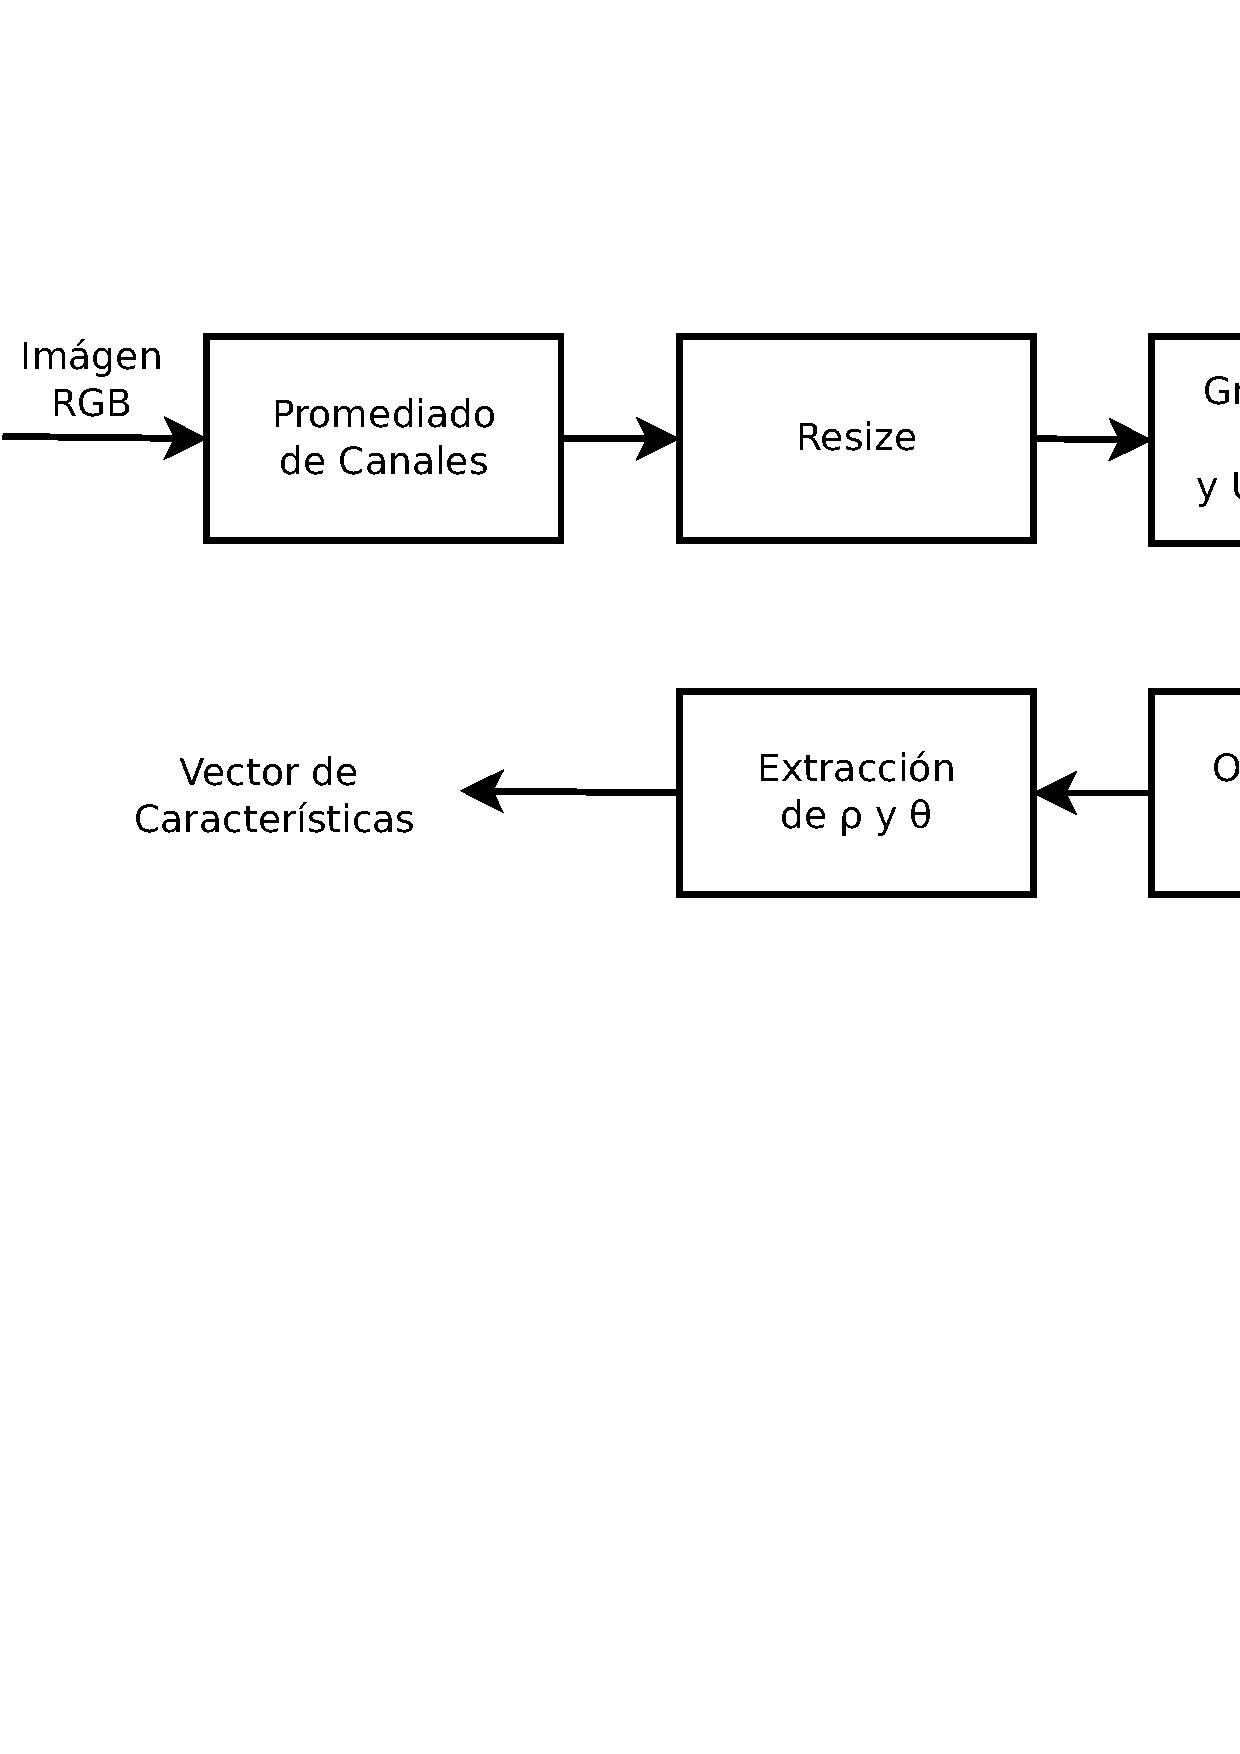
\includegraphics[scale=0.25]{../diagramas/procesohough} 
\end{center}
\caption{Proceso de la imagen mediante el método por T. de Hough}
\label{procesohough}
\end{figure}
%
%%%%%%%%%%%%%%%%%%%%%%%%%%%%%%%%%%%%%%%%%%%%%%%%%%%%%%%%%%%%%%%%%%%%%%%%%%%%%%%%
%
\subsection*{Extracción de características por estadísticas del histograma}
A partir de la imagen original, se normaliza su tamaño y se toman 2 ``perfiles
de intensidad'': uno horizontal, calculado promediando cada columna de la
imagen, y otro vertical obtenido al promediar cada fila. Se obtiene un
histograma para la imagen entera y uno para cada perfil, y se guardan en el
vector de características la media aritmética $m$, mediana $M$ (posición del
percentil 50),  y desviación absoluta $D_{\T{abs}}$ respecto de la mediana:
\begin{equation*}
D_{\T{abs}}=\sum_i |x_i - M|
\end{equation*}
Así se han obtenido un vector de 9 valores que caracterizan histogramas de la
imagen entera.

Luego se subdivide la imagen en cuatro cuadrantes, y se obtienen para cada uno
las mismas medidas que se calcularon para la imagen entera.

Así se obtiene un vector de 45 características a partir de histogramas que se
guardarán en la base de datos para comparación.

\begin{figure}
\begin{center}
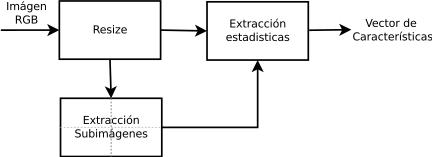
\includegraphics[scale=0.25]{../diagramas/procesoestadisticas} 
\end{center}
\caption{Proceso de la imagen mediante el método de estadísticas del histograma}
\label{procesoestadisticas}
\end{figure}
\begin{figure}
\begin{center}
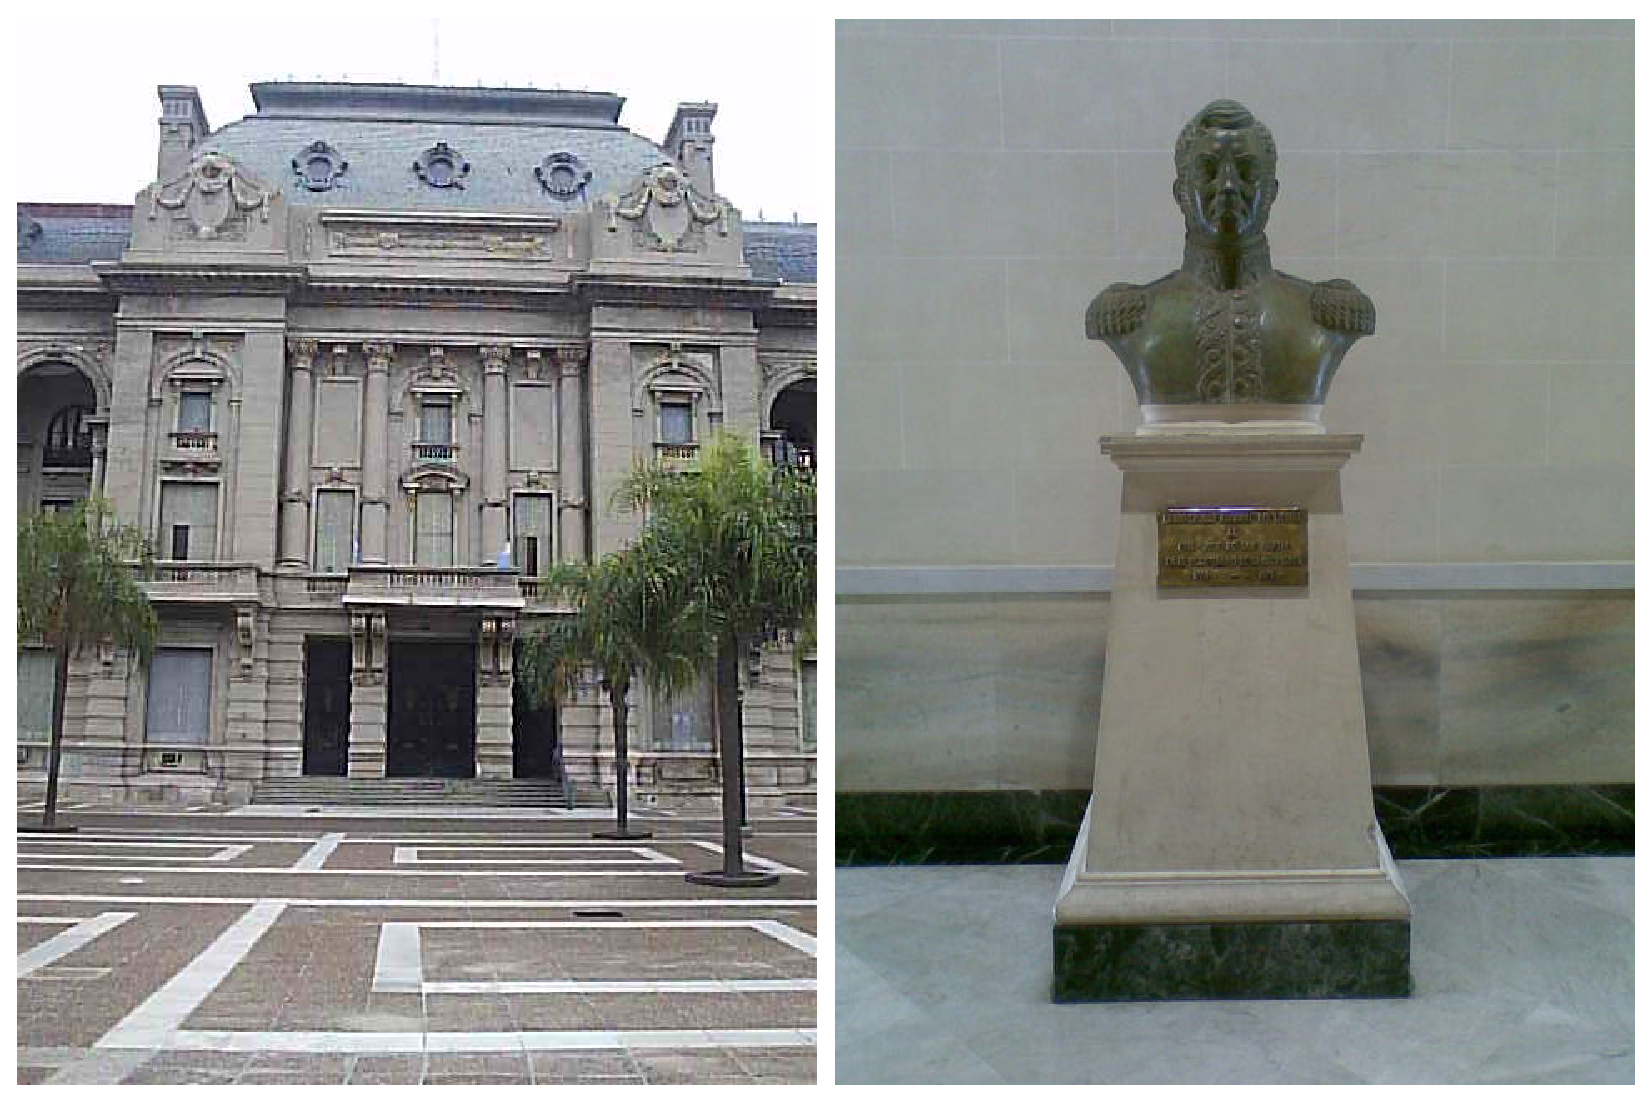
\includegraphics[scale=0.25]{../diagramas/dibujo} 
\end{center}
\caption{Imágenes de pruebas utilizadas con los algoritmos}
\label{imagenes}
\end{figure}
%
%
%%%%%%%%%%%%%%%%%%%%%%%%%%%%%%%%%%%%%%%%%%%%%%%%%%%%%%%%%%%%%%%%%%%%%%%%%%%%%%%%
%
%
\section{Experimentos y resultados}
%
%%%%%%%%%%%%%%%%%%%%%%%%%%%%%%%%%%%%%%%%%%%%%%%%%%%%%%%%%%%%%%%%%%%%%%%%%%%%%%%%
%
\subsection{Descripción de las pruebas}
Para la prueba del método se utilizó validación cruzada, entrenando la base de
datos con 10 imágenes por clase y 3 de prueba por cada clase. Se utilizaron
3 conjuntos de imágenes diferentes, con 5 clases cada uno.

Las imágenes de prueba fueron tomadas con teléfonos celulares corrientes, a una
resolución VGA estándar de 640 píxeles de ancho por 480 de alto, en
diferentes condiciones
de iluminación: día a pleno sol, día nublado, noche, e interior, a monumentos/%
estatuas y edificios en diferentes lugares de la ciudad de Santa Fe, Argentina.
Se muestran en la figura \ref{imagenes} algunos ejemplos.
Los conjuntos se formaron sorteando las 15 clases de imágenes disponibles en
3 de 5 clases cada uno.

Se probaron, en primer lugar, la extracción de características mediante
transformada de Hough y mediante histogramas por separado.

Para el método de Hough se probaron diferentes valores de $U$, el umbral
aplicado a la imagen de bordes, y $N$, el número de máximos en el espacio de
la transformada de Hough a tener en cuenta para armar el vector de $2N$
características.

Para el método de histograma se consideró el histograma del canal de
intensidad en el espacio de colores HSI.

Luego se consideró el rendimiento del método utilizando ambas técnicas en
forma conjunta, para los parámetros de Hough $U$ y $N$ óptimos encontrados.
Se realizó además una prueba para las 15 clases de imágenes en conjunto,
con el objetivo de tener una estimación de cómo escala el método para
mayor número de imágenes.

\subsubsection*{Tasa de error}
Se considera la tasa de error $\%$ del método según:
\begin{equation}
E_\%=100\cdot\frac{\T{número de errores}}{\T{número de pruebas}},
\end{equation}
considerando como error cada prueba en que la imagen es mal etiquetada.

Cabe observar que no se considera como error la vez que el método identifica
una imagen como el monumento acertado, pero en otras
condiciones de iluminación (cuando por ejemplo, la imagen de un monumento
tomada de día es clasificada como la del mismo monumento, pero tomada de noche).
Esta consideración se hace debido a que la detección de bordes elimina la
información de \resalt{luminosidad}  de la imagen; y está claro que no influye
en la clasificación por histograma; ya que éste varía significativamente
entre las versiones de día y noche, en particular, la media y mediana tendrán
valores bastante menores en la imagen nocturna que en aquella tomada de día.
Esto es además consistente con el objetivo del método, que es la correcta
identificación independientemente de las condiciones en que se toma la imagen.
%
% %%%%%%%%%%%%%%%%%%%%%%%%%%%%%%%%%%%%%%%%%%%%%%%%%%%%%%%%%%%%%%%%%%%%%%%%%%%%%%
%
\subsection{Resultados}
\begin{table}
\caption{Tasas de error para métodos}
\begin{center}
\begin{tabular}{ccc}
\hline \emph{Método} & \emph{5 clases} & \emph{15 clases}\\ 
\hline Histogramas & 0\% & 0\%\\ 
\hline Hough & 35.5\% & 60.43\%\\ 
\hline Ambos & 2.22\% & 4.17\%\\ 
\hline 
\end{tabular} 
\end{center}
\label{tablaerrores}
\end{table}

Los resultados de las pruebas para el método de Hough se muestran en la figura
\ref{graficaerror}. Se ha tomado un rango de valores representativos de $U$
y $N$ basados en pruebas previas, donde hemos identificado regiones de mínimo
error para $U~\in(60,120)$ y $N~\in(20,60)$.
En la misma figura se puede apreciar que la tasa de error mínima se obtuvo
para un umbral $U = 100$ y unos $N = 30$ máximos (en promedio).
%
%Debemos comentar aquí que para el método de Hough se realizaron una serie de pruebas
%que determinaron el rango representativo a analizar (umbral $U$ entre 60 y 120 y cantidad
%de máximos $N$ entre 20 y 60). 
En la tabla \ref{tablaerrores} se presentan los resultados para las pruebas
iniciales con conjuntos de 5 clases, y la estimación del resultado con
15 clases. 
%Cabe aclarar que en el primer caso se tomó un promedio de los errores
%sobre el conjunto.

Se puede observar que para el método de histogramas la tasa de error fue cero en
ambas pruebas. En tanto que para el método de Hough se obtiene menor tasa de
error con el conjunto de 5 clases que con el de 15 de 35.5\% y 60.43\%
respectivamente.
En la última fila se muestran los resultados de considerar ambos criterios
en conjunto, asignándole un peso equivalente a cada uno. 

\begin{figure}
\begin{center}
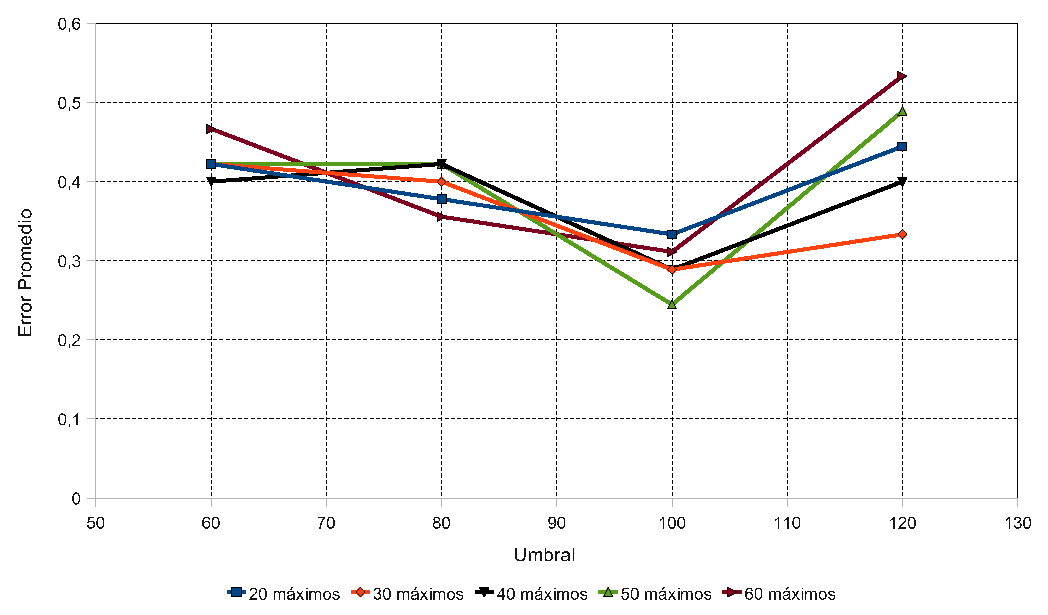
\includegraphics[width=8.5cm]{../diagramas/estadistica_noche_iguales} 
\end{center}
\caption{Error de clasificación promedio en función de distintos $U$ y $N$ para
el método de Hough.}
\label{graficaerror}
\end{figure}
%
% %%%%%%%%%%%%%%%%%%%%%%%%%%%%%%%%%%%%%%%%%%%%%%%%%%%%%%%%%%%%%%%%%%%%%%%%%%%%%%
%
\subsection{Discusión}
A pesar de la muy buena performance del método de histograma, debemos tener
presente que los conjuntos de imágenes de entrenamiento/prueba para el método
han sido obtenidas en todos los casos a partir de una secuencia tomada en el 
lapso de unos minutos, lo cual implica que las condiciones de iluminación en
cada conjunto son prácticamente iguales. 

Los histogramas miden la distribución estadística de los diferentes niveles
de intensidad presentes en la imagen, luego están estrechamente relacionados
con las condiciones de iluminación de la escena. Por este motivo, tenemos
que los histogramas entre las imágenes de entrenamiento/prueba son, a los
efectos prácticos, idénticos, lo cual explica el buen funcionamiento de este
método.

Se ha probado la técnica de histogramas sobre el canal I del espacio de color
HSI; por lo antes expuesto, debemos tener en cuenta consideraciones similares
para el resto de los canales de la imagen.

En general, se deberá poner énfasis en definir técnicas
de ``normalización'' orientadas a mejorar los resultados en condiciones más
realistas. Se deberá considerar la utilización de métodos de histograma
mejorados, por ejemplo el \emph{histograma de combinación espacial de DCT
ponderada} \cite{wdctsch}, \emph{vectores de coherencia de
color} \cite{Pass96histogramrefinement}, o el procesamiento de
histogramas borrosos presentado en \cite{Konstantinidis2005375}.

Respecto de la extracción de características mediante la transformada de Hough,
vemos que el rendimiento no es tan bueno como en la técnica de histogramas,
sin embargo en varios casos ha sido capaz de identificar correctamente edificios
a pesar de las diferentes condiciones de iluminación (día y noche), el cual
 es un resultado alentador.

No podemos evitar la mención al costo computacional del proceso, que aunque
no es tan elevado como para considerar impráctico el método, sí será una
limitante al considerar implementaciones en tiempo real o de alta velocidad
de respuesta: en una computadora promedio el cálculo se realiza en 1-2 segundos,
luego es esperable que este tiempo se triplique en un dispositivo móvil.

Se deberá considerar la utilización de un detector de bordes como el propuesto
por Canny \cite{canny}, así como tambien técnicas de preprocesamiento de la
imagen, como puede ser el filtrado homomórfico, en pos de mejorar los
resultados obtenidos en nuestras pruebas.

En lo que respecta a la escalabilidad de la base de datos, los resultados no
son particularmente alentadores, lo que nos obliga a considerar otra vez la
utilización de métodos más refinados de histograma y transformada de Hough.
%
%
% %%%%%%%%%%%%%%%%%%%%%%%%%%%%%%%%%%%%%%%%%%%%%%%%%%%%%%%%%%%%%%%%%%%%%%%%%%%%%%
%
%
\section{Conclusiones}
Se ha presentado una técnica para la identificación de edificios, monumentos,
esculturas con extracción de características mediante medidas de histograma
y transformada de Hough.

El rendimiento ha sido satisfactorio considerando las restricciones a las
que se han sometido las pruebas.

Se deberá optimizar la implementación para portarlo a dispositivos móviles
con capacidad de procesamiento limitada.

Se hace necesario el preprocesamiento de la imagen, así como la incorporación
de métodos más refinados de extracción de características, para mejorar los
resultados obtenidos y así poder escalar el método a una base de datos de
mayor magnitud.
%
%
% %%%%%%%%%%%%%%%%%%%%%%%%%%%%%%%%%%%%%%%%%%%%%%%%%%%%%%%%%%%%%%%%%%%%%%%%%%%%%%
%
%
\section{Trabajos futuros}
A partir del diseño aquí presentado, nos proponemos continuar
investigando esta técnica considerando las siguientes posibilidades:
\begin{itemize}
\item Aplicación de filtrado homomórfico y otros tipos de
      pre-procesamiento en las imágenes.
\item Aplicación de técnicas de \eng{warping} y otras transformaciones en busca
      de lograr invarianza respecto de rotación y escalado de la imagen.
\item Desarrollo de una implementación óptima para dispositivos móviles con
      poder de procesamiento limitado.
\item Desarrollo de técnicas de extracción de características más robustas que
      las aquí presentadas.
\end{itemize}
\nocite{*}
\bibliographystyle{tfmpd}
\bibliography{tfmpd}
\end{document}
